\documentclass[12pt]{article}
\usepackage{sbc-template}
\usepackage[utf8]{inputenc}
\usepackage[portuguese]{babel}
\usepackage{lipsum} 
\usepackage{graphicx,url}
\usepackage{amsmath,bm,bbm}\usepackage{natbib}
\usepackage[colorlinks=true, allcolors=blue]{hyperref} 

\sloppy

\title{Clusterização de texturas de Broadtz no plano HC}

\author{Alejandro Frery\inst{1}, Osvaldo Rosso\inst{1}, Eduarda Chagas\inst{2}}


\address{
  Laboratório de Computação Científica e Análise Numérica (LaCCAN)\\
  Universidade Federal de Alagoas (UFAL) -- Maceio, AL -- Brazil
  \nextinstitute
  Departamento de Ciência da Computação\\
  Universidade Federal de Minas Gerais (UFMG) -- Belo Horizonte, MG -- Brazil
  \email{eduardachagas48@laccan.ufal.br}
}

\begin{document}

\maketitle

\section{Introdução}

Em análises anteriores foi levantada a hipótese de que ao realizar a caracterização das texturas de Broadtz no plano Complexidade-Entropia alguns clusters eram formados, dividindo os dados em subconjuntos.

Foram analisadas um total de $45$ texturas e seus respectivos pontos no plano, para todas as combinações entre o conjunto de dimensões $\bm D = \{2,3,4,5,6\}$ e delay $\bm \tau = \{1,2,3,4,5\}$. Como podemos verificar na Figura~\ref{fig:textureshC}, os planos $(\bm D = 5, \bm \tau = 1)$, $(\bm D = 5, \bm \tau = 2)$, $(\bm D = 5, \bm \tau = 3)$ e $(\bm D = 5, \bm \tau = 4)$ separaram visualmente os dados em três subconjuntos. Entretanto, nenhuma análise experimental havia sido feito para comprovar tais suposições. 

\begin{figure}[!h]
	\centering
	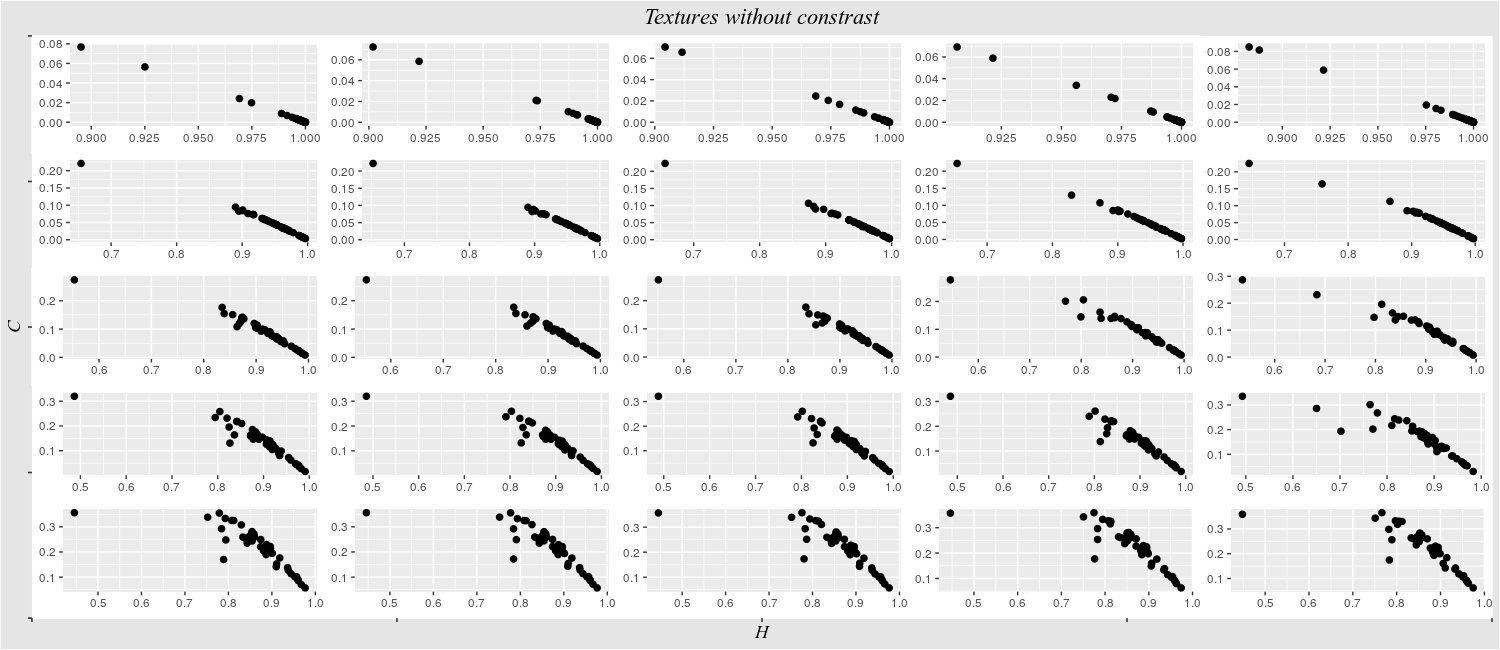
\includegraphics[scale = 0.42]{../../Images/Textures/Textures_no_contrast.png}   
	\caption{Texturas de Broadtz mapeadas no plano $\mathcal H\times \mathcal C$}
	\label{fig:textureshC}
\end{figure}

Desse modo, descreveremos brevemente como foi realizado esse estudo e quais resultados foram adquiridos com o mesmo.

\begin{figure}[!h]
	\centering
	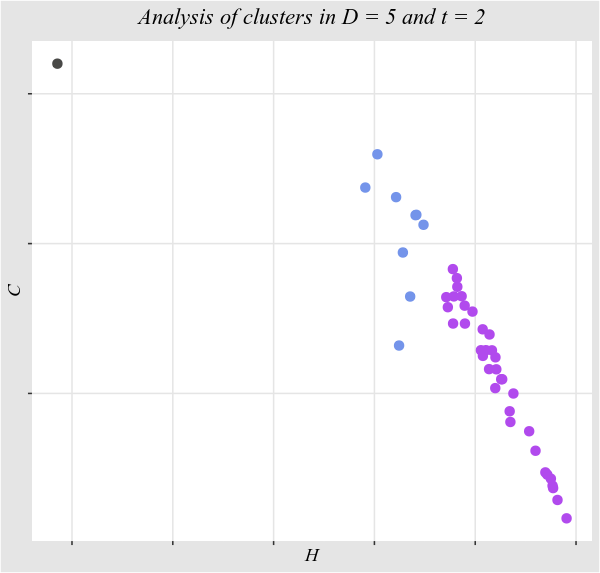
\includegraphics[scale = 0.6]{../../Images/Textures/cluters_textures.png} 
	\caption{Clusters visualmente formados no plano $\mathcal H\times \mathcal C$}
	\label{fig:clusters}
\end{figure}

\newpage

\section{Metodologia}

O primeiro passo foi escolher um método de agrupamento que fosse adequado para o problema apresentado. 
Assim, algumas características e apontamentos foram levados em consideração durante a escolha, foram eles:

\begin{itemize}
    \item Queremos encontrar uma técnica eficiente e eficaz na detecção de clusters "naturais" e seus arranjos no plano $\mathcal H\times \mathcal C$;
    \item Não possuímos nenhuma informação prévia dos grupos que podem ser formados, logo trata-se de um estudo de aprendizagem não supervisionada;
    \item Os clusters podem ter formatos arbitrários e diferentes tamanhos.
\end{itemize}

Sabendo disto, optamos por escolher o algoritmo \texttt{DBSCAN} para realizar o agrupamento dos descritores, que se trata de uma método não-paramétrico baseado em densidade.
O funcionamento do algoritmo se baseia na ideia de que para cada ponto de um certo cluster, a vizinhança para um dado raio contém, no mínimo, um determinado número de pontos, isto é, a densidade da vizinhança tem que exceder um limiar.

Para isso, utilizamos o pacote \texttt{dbscan} para aplicar a técnica nos dados dos descritores e a configuramos, de modo empírico, com os seguintes valores:

\begin{itemize}
    \item Semente $123$;
    \item Tamanho da vizinhança $\epsilon = 0.035$;
    \item Número mínimo de pontos na região $2$.
\end{itemize}

\section{Resultados e conclusões}

Após aplicar o \texttt{DBSCAN} conseguimos verificar a formação de alguns clusters nos planos, como podemos ver na Figura~\ref{fig:dbscan}.

\begin{figure}[!h]
	\centering
	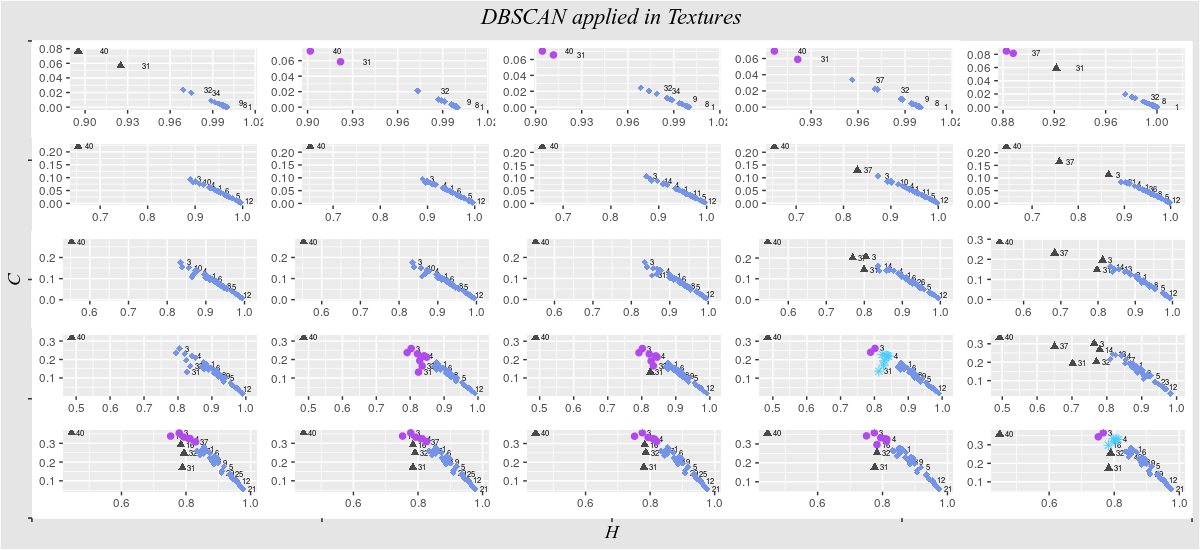
\includegraphics[scale = 0.42]{../../Images/Textures/DBSCAN.png} 
	\caption{Clusters formados no plano $\mathcal H\times \mathcal C$ pelo algoritmo DBSCAN}
	\label{fig:dbscan}
\end{figure}

Como resultado, vemos que os planos $\mathcal H\times \mathcal C$ $(\bm D = 5, \bm \tau = 2)$, $(\bm D = 5, \bm \tau = 3)$ e $(\bm D = 5, \bm \tau = 4)$ nos mostram que os dados podem ser separados em dois ou até três subgrupos de texturas com comportamento similares.  

Possuímos agora como trabalhos futuro verificar se os grupos formados com o algoritmo possuem alguma informação semântica similar, nos revelando alguma característica relevante acerca da dinâmica dos seus elementos.

\end{document}